\documentclass[12pt]{book}

%\usepackage{cvs-support}
\usepackage{varioref,listings,array,subfigure,makeidx,fancyhdr,amsfonts,url,vmargin,color}
\usepackage[pdftex]{graphicx}
\usepackage{caption2}
%\usepackage[longfirst]{glosstex}
\usepackage[Sonny]{fncychap}


\usepackage[pdftex,letterpaper=true,pagebackref=false]{hyperref} % with basic options
		% N.B. pagebackref=true provides links back from the References to the body text. This can cause trouble for printing.
\hypersetup{
    plainpages=false,       % needed if Roman numbers in frontpages
    pdfpagelabels=true,     % adds page number as label in Acrobat's page count
    bookmarks=true,         % show bookmarks bar?
    unicode=false,          % non-Latin characters in Acrobat’s bookmarks
    pdftoolbar=true,        % show Acrobat’s toolbar?
    pdfmenubar=true,        % show Acrobat’s menu?
    pdffitwindow=false,     % window fit to page when opened
    pdfstartview={FitH},    % fits the width of the page to the window
    pdftitle={uWaterloo\ LaTeX\ Thesis\ Template},    % title: CHANGE THIS TEXT!
%    pdfauthor={Author},    % author: CHANGE THIS TEXT! and uncomment this line
%    pdfsubject={Subject},  % subject: CHANGE THIS TEXT! and uncomment this line
%    pdfkeywords={keyword1} {key2} {key3}, % list of keywords, and uncomment this line if desired
    pdfnewwindow=true,      % links in new window
    colorlinks=true,        % false: boxed links; true: colored links
    linkcolor=blue,         % color of internal links
    citecolor=green,        % color of links to bibliography
    filecolor=magenta,      % color of file links
    urlcolor=cyan           % color of external links
}


\setlength\captionindent{2mm}
\renewcommand*\captionfont{\sf \small}
\renewcommand*\captionlabeldelim{.\hspace*{.5cm}}

\renewcommand*\captionlabelfont{\sf \it \small}


\newcommand{\HRule}[1]{\rule{\linewidth}{#1}}
\newcommand{\ltwo}{L$^{2}$ }
\newcommand{\family}[1]{\emph{#1}}

\newcommand{\method}[1]{\textsf{\small #1}}
\newcommand{\no}{{\bfseries -}}
\newcommand{\yes}{$\surd$}
\newcommand{\well}{$\approx$}
\newcommand{\na}{\bfseries n/a}
\newcommand{\auto}{\textbullet}
\newcommand\uc[1]{\textsf{\small #1}}


\setlength{\parskip}{8pt}
\graphicspath{{fig/}}

%%%%%%%%%%%%%%%%%%%%%%%%%%%%%%
%% AFTER \begin{document}
%%%%%%%%%%%%%%%%%%%%%%%%%%%%%%
\begin{document}
\thispagestyle {empty}
\vspace*{\stretch{1}}

%\HRule

\begin{center}
\noindent \HRule{1.5mm} \\[5mm]

  \noindent \normalsize \textbf{Real-Time Embedded Software Group} \\[2mm]
    \noindent \Large \textbf{RiTHM: A Tool for Enabling Time-triggered Runtime Verification for C Programs}\\[4mm]
    \noindent \large User's Guide

  \noindent \HRule{1.5mm}

  \vspace*{2cm}




  \vspace*{\stretch{1}}

  Electrical and Computer Engineering Department, \\University of Waterloo, January 2013\\

  \end{center}


  % \begin{minipage}{\textwidth}
  % \flushright
  % {\bfseries
  %   \Large
  % Sebastian Fischmeister\\[1.5ex]
  % }
  % \end{minipage}

  % \vspace*{\stretch{2}}


  %   \begin{center}
  %     \Large \textbf{Sebastian Fischmeister} \\
  %     \large Fischmeister@SoftwareResearch.net \\[-1mm]
  %     \large Department of Computer Science \\[-1mm]
  %     \large Software Research Lab \\[-1mm]
  %     \large University of Salzburg \\[-1mm]
  %     \large A-5020 Salzburg, Austria
  %   \end{center}

  %   \vspace*{1cm}

  %   \begin{center}
  %     under guidance of \\
  %     \Large \textbf{Prof. Dr. Wolfgang Pree} \\
  %     \large Pree@SoftwareResearch.net \\[-1mm]
  %     \large Department of Computer Science \\[-1mm]
  %     \large Software Research Lab \\[-1mm]
  %     \large University of Salzburg \\[-1mm]
  %    \large A-5020 Salzburg, Austria
  %   \end{center}


  % \begin{minipage}{\linewidth}
  % \footnotesize
  % \textbf{Revisions:} \\
  % \listofrevisions
  % \end{minipage}

  %\indent \emph{Titlepage:} $Revision: 1.7 $ \\
  %\indent \emph{Concepts of Mobile Computing and
  %Context-Awareness:} \revConceptsofMobileComputing

  %\HRule

  \newpage

\pagestyle{plain}
\setcounter{page}{2}
\pagenumbering{roman}

% T A B L E   O F   C O N T E N T S
% ---------------------------------
\renewcommand\contentsname{Table of Contents}
\tableofcontents
\cleardoublepage
\phantomsection
%\newpage

% L I S T   O F   T A B L E S
% ---------------------------
\addcontentsline{toc}{chapter}{List of Tables}
\listoftables
\cleardoublepage
\phantomsection		% allows hyperref to link to the correct page
%\newpage

% L I S T   O F   F I G U R E S
% -----------------------------
\addcontentsline{toc}{chapter}{List of Figures}
\listoffigures
\cleardoublepage
\phantomsection		% allows hyperref to link to the correct page
%\newpage

% L I S T   O F   S Y M B O L S
% -----------------------------
% To include a Nomenclature section
% \addcontentsline{toc}{chapter}{\textbf{Nomenclature}}
% \renewcommand{\nomname}{Nomenclature}
% \printglossary
% \cleardoublepage
% \phantomsection % allows hyperref to link to the correct page
% \newpage

% Change page numbering back to Arabic numerals
\pagenumbering{arabic}

\pagestyle{fancy}
%\addtolength{\headwidth}{\marginparsep}
%\addtolength{\headwidth}{\marginparwidth}
\renewcommand{\chaptermark}[1]{\markboth{#1}{}}
\renewcommand{\sectionmark}[1]{\markright{\thesection\ #1}}
\fancyhf{}
\fancyhead[LE,RO]{\small\bfseries\thepage}
\fancyhead[LO]{\footnotesize\bfseries\rightmark}
\fancyhead[RE]{\footnotesize\bfseries\leftmark}
\fancypagestyle{plain}{%
\fancyhead{} % get rid of headers
\renewcommand{\headrulewidth}{0pt} % and the line
}

\chapter*{About This Guide}
This guide is intended for software developers that wish to contribute to RiTHM, which is a toolchain targeted to automate the process of deploying time-triggered monitors for runtime verification of projects that are written in C. The rest of the guide will describe the process of pulling and building the toolchain source and a brief description of the repository directory structure, mapping it to RiTHM's internal components.

\chapter{Getting Started}
This chapter will guide you through the procedure to download RiTHM's source files and build the tool from source. At the time of writing, RiTHM is targeted for both 32- and 64-bit Ubuntu 12.04 LTS. Most of the build and execution infrastructure should be portable to any *nix systems, but will require additional efforts to build RiTHM's dependencies. Other *nix distributions may be supported in the future.

\section{Pre-requisites}
The following is a list of things that you will require to build and develop RiTHM:
\begin{itemize}
	\item A computer running Ubuntu 12.04 LTS
	\item {\tt sudo} access with your user account in Ubuntu
	\item {\tt git} installed on your machine. If {\tt git} has not been installed on your machine, you can install it in            Ubuntu by typing the following command in
           the terminal:
           \begin{center}
           	{\tt sudo apt-get install git}
           \end{center}
	\item Bitbucket account (this is optional; you can choose to download the source and work locally)
	\item SSH keys, if you wish to connect to Bitbucket via SSH
	\item Text editor of your choice
	\item An integrated development environment (IDE) if you are not as comfortable with the command line
\end{itemize}

\section{Acquiring and Building the Source Files}
\noindent \textbf{Step 1.} \ To work with the git repository on Bitbucket, first, log into your Bitbucket account in a web browser. Then, visit the
following webpage:
\begin{center}
	\url{https://bitbucket.org/embedded_software_group/rvtool}
\end{center}
Within the webpage, find the button that is labeled as `Fork'. Figure~\ref{fig:bitbucket-fork} shows where this button is located. Click on the button and fill out the necessary fields in the form that is presented to you. Once you are done filling out the form, Bitbucket will effectively make a copy of the tool repository under your account.

\begin{figure}[t]
	\centering
	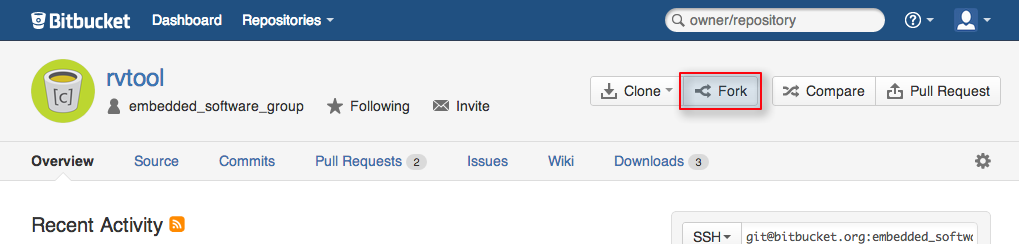
\includegraphics[width=0.9\textwidth]{bitbucket-fork}
	\caption[Screenshot of Bitbucket web interface.]{Screenshot of Bitbucket web interface. The red box highlights where the `Fork' button is.}
	\label{fig:bitbucket-fork}
\end{figure}


\noindent \textbf{Step 2.} \ Once you have successfully forked the repository, you can clone the repository to your local machine. If you plan on using HTTPS to communicate with the remote Bitbucket repository, change to the directory that you would like to make your clone in and then enter the following command in terminal:
\begin{center}
	{\tt git clone https://<username>@bitbucket.org/<username>/<name of forked repository>.git [name of local directory]}
\end{center}
where {\tt <username>} is you Bitbucket username, {\tt <name of forked repository>} is the name you gave the forked repository in the forking step, and an optional argument {\tt [name of local directory]}, which designates the name of the folder the cloned repository will be in. The {\tt git clone} command is slightly different for SSH:
\begin{center}
	{\tt git clone git@bitbucket.org:<username>/<name of forked repository>.git [name of local directory]}
\end{center}

\noindent \textbf{Step 3.} \ After cloning the forked repository to your local machine, it is time to start building the tool from source. First, change the directory in your terminal to the base repository directory. Here, there are two files you will need to invoke to build the tool:
\begin{itemize}
	\item {\tt build-deps.sh}
	\item {\tt Makefile}
\end{itemize}

{\tt build-deps.sh} contains the necessary commands required to pull in all of the tool's external dependencies and build them as necessary. This will also establish the subdirectory named `build', which will contain all compiled objects and executables. From the terminal, run the following command
\begin{center}
	{\tt sudo ./build-deps.sh}
\end{center}
{\tt sudo} access is required only to install missing packages using {\tt apt-get}. The following packages may be installed using {\tt apt-get}:
\begin{description}
	\item[realpath]: converts any relative directory/file paths into absolute paths
	\item[subversion]: version control required to pull LLVM and Clang source
	\item[ia32-libs]: needed for machines running 64-bit Ubuntu for compatibility with other libraries
\end{description}

This script will likely take one or more hours to finish, because the LLVM framework and Clang takes a long time to compile and build for the first time.

All but one external dependencies are pulled in automatically with this script. The following should be configured and built inside the `build' directory after the script finishes:
\begin{itemize}
	\item realpath
	\item subversion
	\item ia32-libs
	\item libconfig
	\item AMD APP SDK (Note: this is installed in {\tt /opt/AMDAPP/} as opposed to the `build' directory)
	\item LLVM and Clang
	\item Qt and QMake
	\item lp\_solve
\end{itemize}


The only external tool that RiTHM uses that needs to be downloaded separately and installed in the build directory is {\tt yices}:
\begin{center}
	\url{http://yices.csl.sri.com/download.shtml}
\end{center}
Select the distribution that is the most appropriate for your machine. After downloading the archived package, untar the file to the following directory: {\tt <local repository root>/build/solvers/yices}. Manually make the directories if they do not already exist.

When the {\tt build-deps.sh} script has finished running, simply type {\tt make} to build the tool. When make is finished running, you can change to the `build' directory and run RiTHM by using the shell script {\tt run.sh} or the graphical user interface (GUI) {\tt rvtool}. For more details about running RiTHM, please refer to RiTHM's user manual.


\chapter{Repository Structure}

\end{document}


